\documentclass[12pt]{article}

\usepackage[a4paper, hmargin=1in, vmargin={0.5in, 1in}]{geometry}
% \usepackage{fullpage}
\usepackage{amsmath,amssymb}
\usepackage{soul}
\usepackage{bussproofs}
% \usepackage{qtree}
\usepackage{graphicx}
\usepackage{dsfont}
\usepackage{multicol}
\usepackage{hyperref}
\usepackage{listings}
\usepackage{mathtools}


% \setlength{\headheight}{14.0pt}
\bibliographystyle{acm}



\makeatletter
\newcommand*\wrapletters[1]{\wr@pletters#1\@nil}
\def\wr@pletters#1#2\@nil{#1\allowbreak\if&#2&\else\wr@pletters#2\@nil\fi}
\makeatother

% \hypersetup{
%     colorlinks=true,
%     linkcolor=blue,
%     filecolor=magenta,      
%     urlcolor=blue
% }

\title{Drapery: a Cloth Simulation Framework for Minecraft}
\author{Samantha Sussman-Randall}
\date{April 2025}

\begin{document}

\maketitle

\begin{center}
    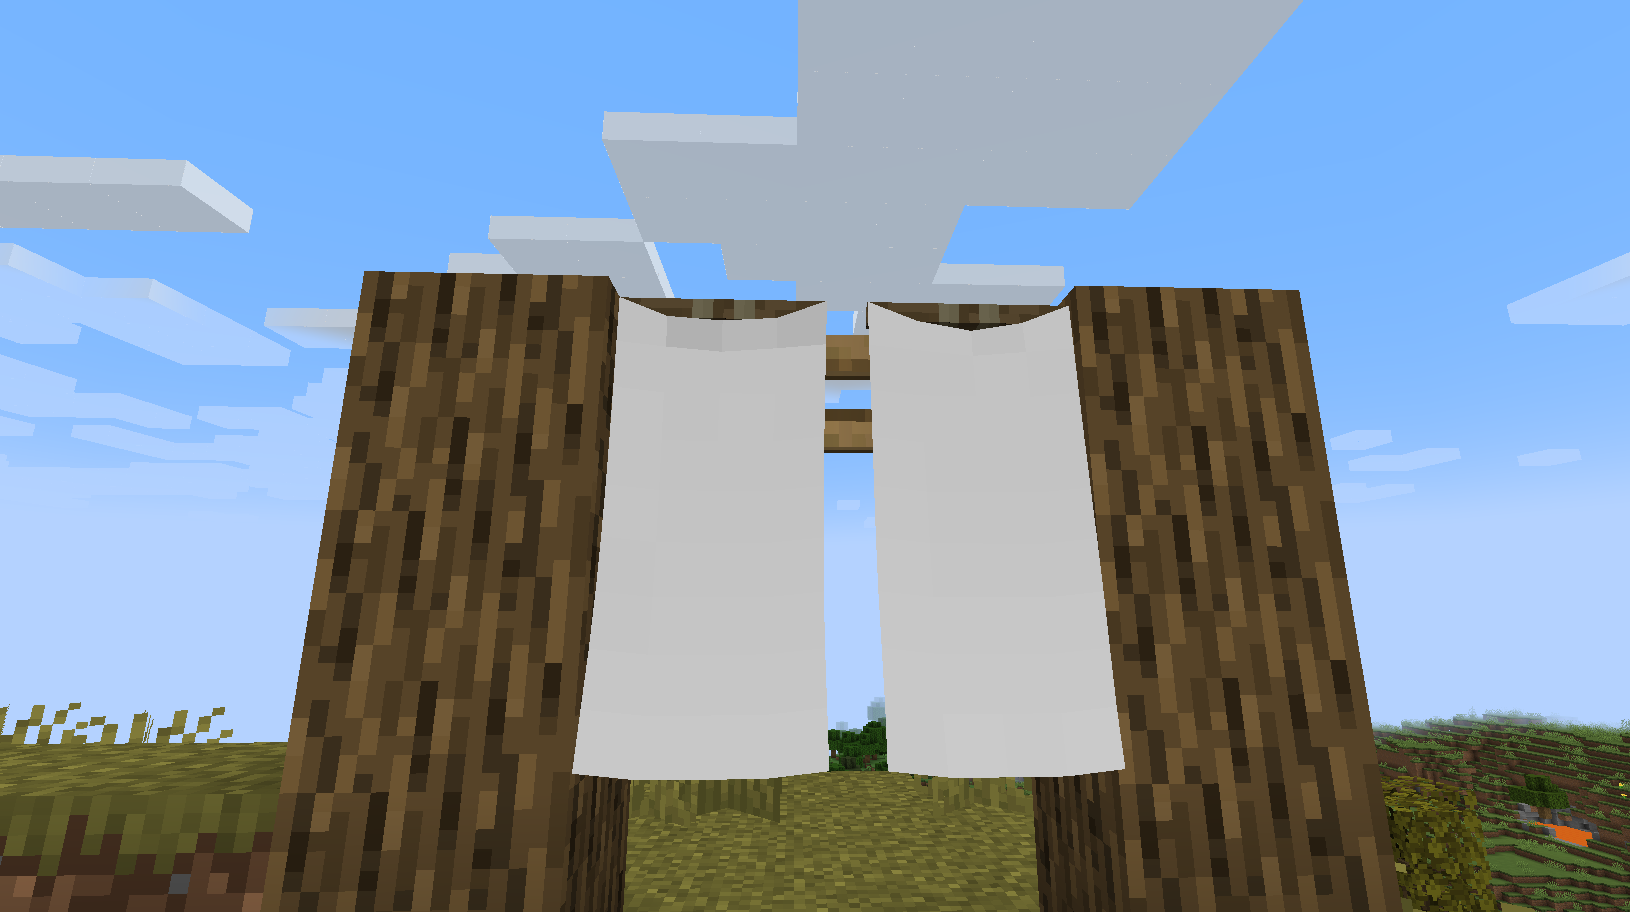
\includegraphics[width=5in]{images/bannerthin.png}
\end{center}

\section{Abstract}

This project makes steps towards a cloth simulation library mod for Minecraft, tentatively named Drapery. Specifically implementing Desbrun, Schröder, and Barr's implicit integration approximation algorithm for mass-spring cloth simulations in Java. As a primary test case, we replace the game's banner renderer with our cloth simulation and find that it produces satisfying realtime results without much impact on game performance. We also discuss previous Minecraft cloth works and how in-game cloth can best match the game's art style.

\section{Motivation}

Minecraft is a popular game with an incredibly active modding scene. Some mods aim to provide new experiences to the game, while others are libraries abstracting out common or more complex logic that other mods can then rely on. While there are some (but not many) mods that use cloth simulations, there are no libraries. The goal here is to make progress towards making one.\\
\\
Adjacently, there will need to be concrete test uses of the library, which gives us a chance to explore what cloth can and should look like in the game's art style.

\section{Related Work}

We'll\footnote{I tend to prefer using 'we' in my writing, I am the only author though. Feel free to consider yourself, the reader, a part of 'we'.} start with a quick review of past cloth simulation methods, then we'll look at past Minecraft-related cloth work for style guidance.

\subsection{Previous Cloth Simulation Methods}

First we have Provot's 1995 work \cite{Provot1995:17} introducing the mass-spring model with constraints to prevent over-stretching. It uses explicit integration and therefore requires very small timesteps.\\
\\
Next came Baraff \& Witkin's Large Steps in Cloth Simulation \cite{largesteps} where they implement implicit integration allowing for stable simulation of larger time steps. This allows computing the same simulation time frame with fewer passes. They also introduce inverse mass matrix modification to constraint individual particles.\\
\\
Desbrun, Schröder, and Barr followed the next year \cite{interanim} with a two step predictor-corrector method that approximates implicit integration without solving a linear system each step and then corrects it similarly to Provot. This method runs faster than Baraff \& Witkin's and they've (somewhat) helpfully included pseudocode for it as well.\\

\subsection{Minecraft Specific Work}

Let's start with Minecraft itself. The game has two cloth-like bits, capes and banners, but I wouldn't quite call them cloth simulations. The cape is a stiff 1 pixel thick rectangular prism that is attached to the player's shoulders and lags behind the players movement. If the player is running forward it'll fly up slightly, if they are falling it'll fly up a lot, if they turn it'll take a second to turn. The banner is similarly a stiff 1 pixel thick rectangular prism that can be hung from a pole or wall. It has a slight swaying animation but otherwise does not interact with its environment. In general, base Minecraft has very limited collision, mostly just a single bounding box per entity. There tends to be a lot of clipping and it generally looks fine!\\
\\
The only full in-game cloth simulation I've found is a part of the Physics mod by Haubna \cite{HaubnaPhysics}. We can see in a posted demo \cite{HaubnaCloth} that they added a cloth simulation to the banners, capes, and fishing rods. It's hard to tell from the video but there appears to be some slight instability or artifacting on the banners when the character walks through them, although this could just be the character clipping through. The cloth (cape and banner) is completely thin and seems to have decent resolution, skewing more towards realism than blocky stylization. Unfortunately, the mod is closed source and these features are locked behind the developer's Patreon, so it's unclear how they implemented this, how much is java modding and how much is done with shaders.\\
\\
There is also the cloth simulation done for Falkreon's Scarves mod \cite{Falkreon}. The scarves are completely thin pieces similar to the physics mod, but use textures from the game so they don't feel too out of place.\\
\\
Outside of modding, we have Dryym's wonderful hand-animated model of a character with a dress in a Minecraft style \cite{Dryym}. They use just a couple of intersecting rectangular prisms textured only on certain sides to give the appearance of flowing cloth. I think this lower resolution style, with only a few bend points, looks very good.

\begin{figure}[h]
    \begin{center}
        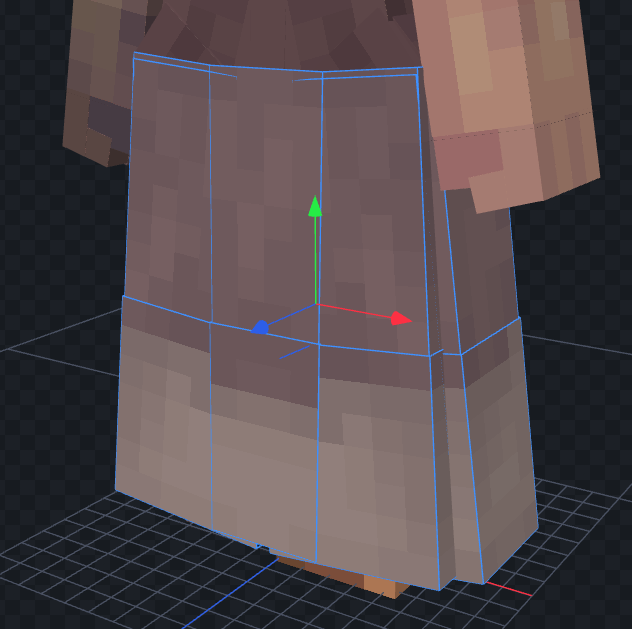
\includegraphics[width=3in]{images/dryym-skirt-blockoutlines-back.png}
    \end{center}
    \caption{Wireframe of Dryym's skirt model}
\end{figure}

\section{Implementation}

\subsection{Cloth Sim Algorithm}

I decided to use the algorithm given in Desbrun, Schröder, and Barr's 1999 paper \cite{interanim} since it seemed fast and simple enough to implement based on the pseudocode given. The four main steps in the algorithm are computing the spring forces, approximating the new velocity, correcting for preservation of angular momentum, and finally running overstretch-correction as in Provot 1995 \cite{Provot1995:17}.\\
\\
This all proved fairly simple, except for the paper's pseudocode containing a typo that derailed about a day of debugging. The paper gives the equation for the spring force on node $i$ by node $j$ as
$$ F_{ij} = k_{ij} (||\mathbf x _i - \mathbf x_j|| - l_0^{ij})\frac{\mathbf x _i - \mathbf x_j}{||\mathbf x _i - \mathbf x_j||}$$
where $\mathbf x_i$ is the current position of node $i$, $l_0^{ij}$ is the rest distance between $i$ and $j$, and $k_{ij}$ is the spring stiffness. When $i$ and $j$ are far apart, we should want them to pull together, so $i$ move towards $j$, but we'd have a positive coefficient attached to a vector pointing from $j$ to $i$, so $i$ is instead pushed away. In the opposite case we get nodes being pulled together when they should be pushed apart, causing the cloth to spiral in on itself as seen in Figure 2. Once this was resolved the simulation stabilized.

\begin{figure}[h]
    \begin{center}
        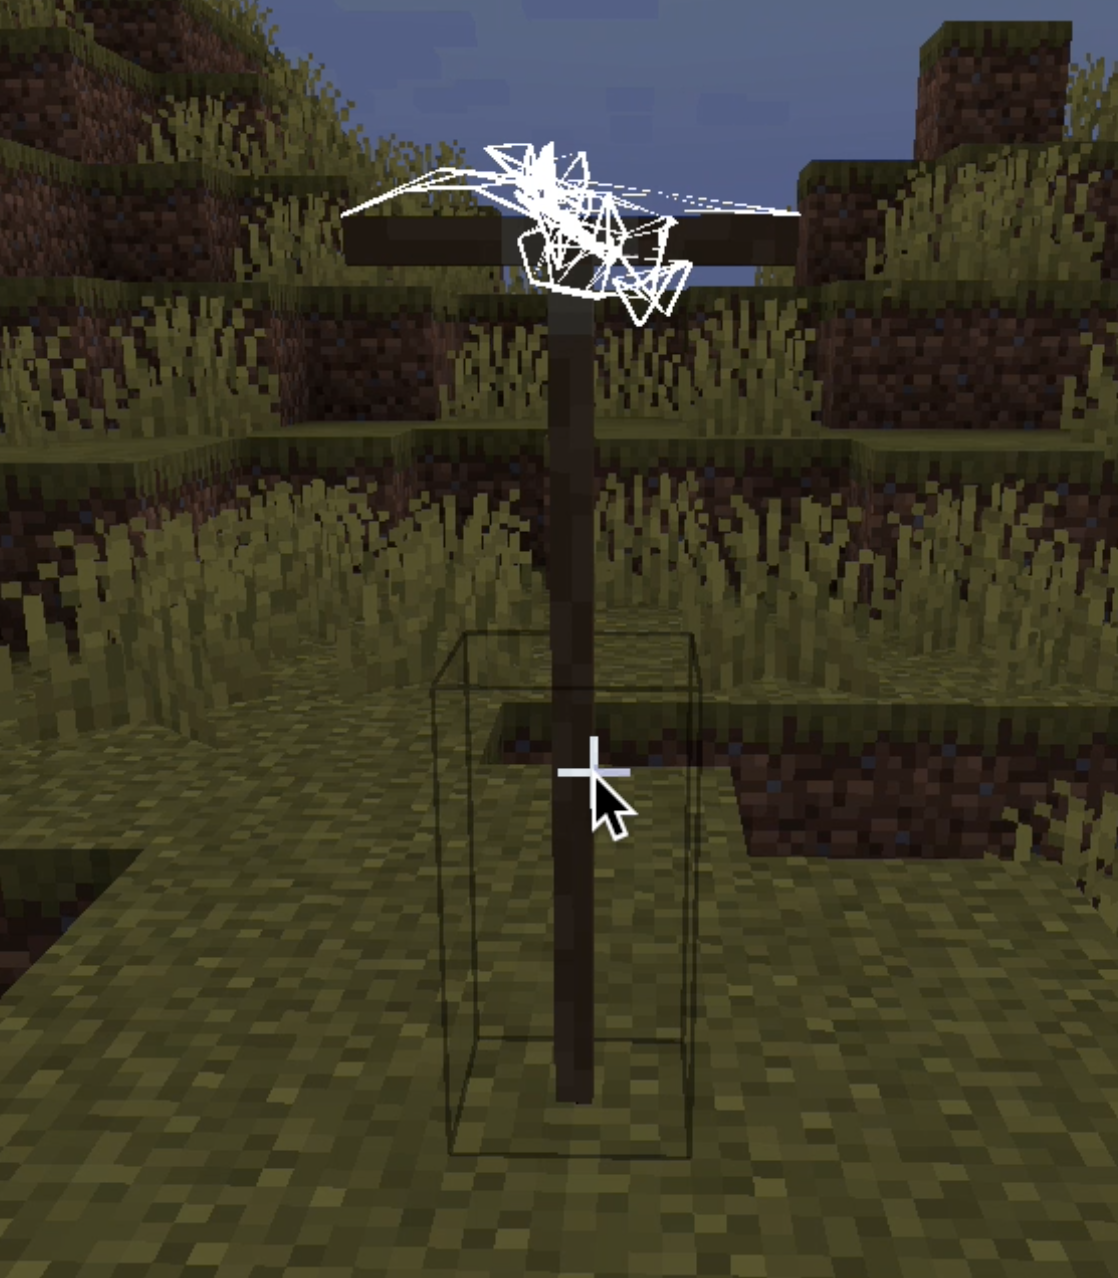
\includegraphics[width=3in]{images/thescrungle.png}
    \end{center}
    \caption{A banner wireframe folding in on itself}
\end{figure}

\subsection{Style Matching}

From our style references, we know that we want to give our cloth a texture, some thickness, and a low mesh resolution. A low mesh resolution is easy enough, just make a smaller grid!\\
\\
We can give the cloth thickness by taking the average normal of each point and moving the vertices to be rendered for that point forward or backward depending on the side. This should give the cloth relatively consistent thickness throughout, maintain UV continuity, and minimize clipping (atleast for non-folded sections).\\
\\
Texturing isn't too hard, except that our primary test case of the banner needs to support multiple texture layers for the decorative patterns, which either need to be rendered as multiple layers or pre-flattened into a single texture. Multiple layers would lead to more quads pushed, while flattening needs to work around the block atlas, and requires some extra care to maintain compatability with common PBR shader formats. I went with multiple layers for simplicity. The UVs were annoying, but that's just how UVs are.\\

\subsection{Mesh Data Structuring}

The current cloth mesh data structuring and general interface is incredibly messy, designed with the primary goal of getting a working environment started to implement the algorithm in. We store a list of immutable particles, which hold information about their original position, UVs, and whether or not they're fixed. Then we store current particle position, velocity, and stiffness in jblas matrices. Finally we store a list of faces to make rendering easier.\\
\\
The mesh constructor takes in a width, height, particle factory, and stiffness factory. This is incredibly unideal, since it locks us to rectangular cloths. Luckily, this is mostly just a problem with the constructor itself, and our simulation, storage, and renderer don't particularly care about the shape of the cloth. The main information we're relying on the rectangular shape for currently is what faces to render.\\
\\
This is also notably quite unoptimized. There's a lot of unnecessary vector copying due to storing data in the matrices, with no real benefit. There's also a good bit of unnecessary looping since we don't have spring lookups. In general a lot of the structuring here should probably be more relational to be more time and memory efficient.

\subsection{Modding Specifics}

The mod is built for Minecraft Java edition version 1.21.1 using the Fabric and NeoForge modloaders and architectury API. It does not currently work for NeoForge, but I believe this is a small gradle issue. The banner renderer is replaced with ours using mixins, which allow us to modify the game's bytecode instructions. Running a single simulation step per frame looks and runs fine enough, there's likely better ways to do it, perhaps on game tick instead.\\
\\
I did not get to collisions or world effects at this point. Giving the banners simple gravity and a slight constant force from behind seems to work well enough to give a convincing swaying effect, although it does eventually reach an equilibrium. Falkreon \cite{Falkreon} uses a sin wave for his wind, likely to get around this and provide a consistent breeze across the world.\\
\\
The banner renderer is currently rather adhoc and hardcoded, which is not ideal, but designing a full and proper API that neatly exposes enough settings is a future task.

\section{Results}

Our cloth banners look pretty good! They run fine in realtime with no notable lag for a reasonable number of banners. They don't quite look blocky yet, though implementing the normal extrusion will likely help with that.\\
\\
As a stress test I made a banner cube with 4913 banners rendering at once, which was incredibly laggy, but still interactive! The simulation can be a bit choppy for larger grid sizes though. With further optimizations, such as LOD distance checks, hard limits on simulations running at once, and improving the mesh structure and algorithm performance as mentioned before, I believe this can run fine in realtime. Dealing with collisions in the future may pose a challenge to performance, but we have the benefit of not going for realism, so we can hopefully keep our collision checks minimal.
\begin{figure}[hp]
    \begin{center}
        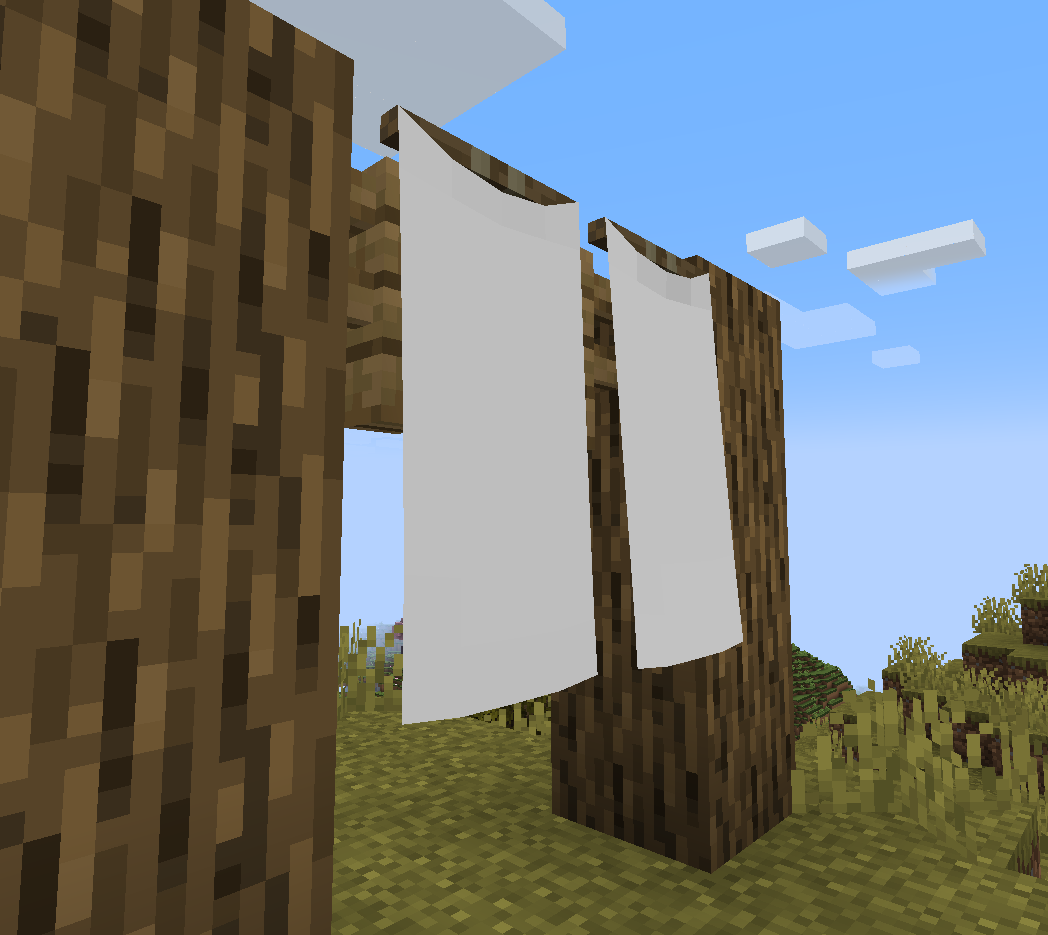
\includegraphics[height=2.75in]{images/bannersflowy.png}
        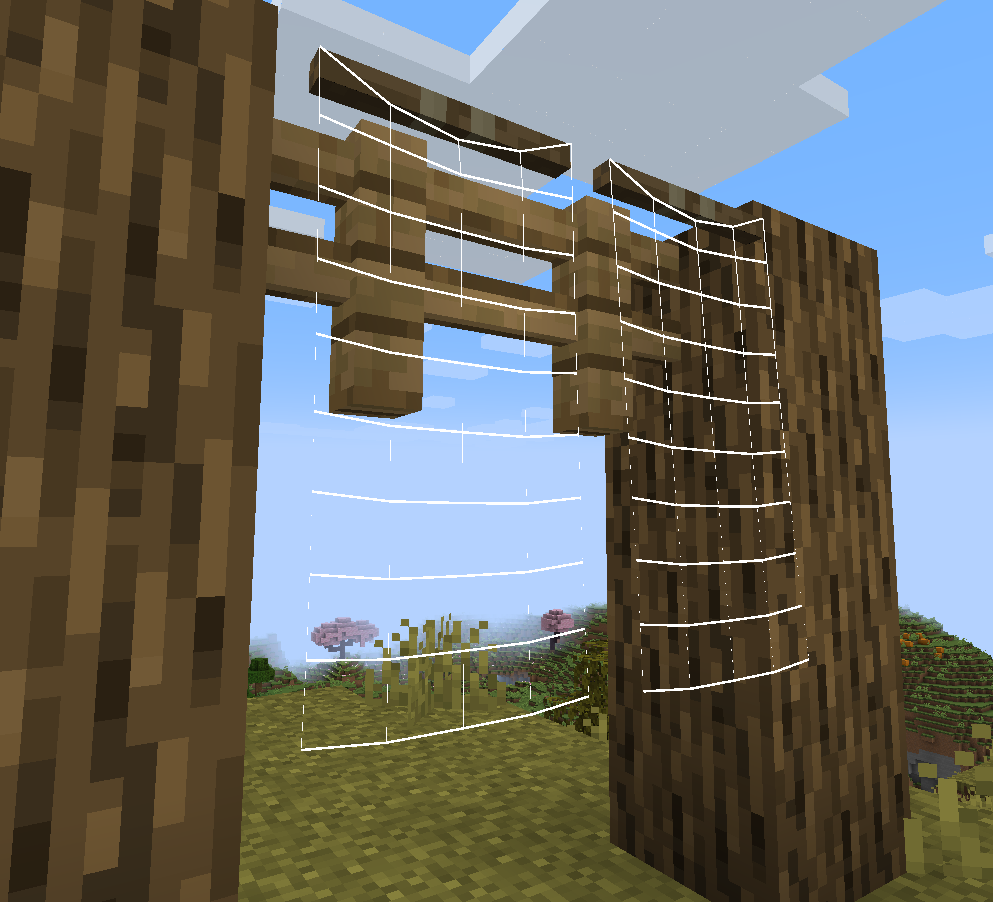
\includegraphics[height=2.75in]{images/bannersflowywireframe.png}
    \end{center}
    \caption{Banners with relatively small grids.}
\end{figure}

\begin{figure}[hp]
    \begin{center}
        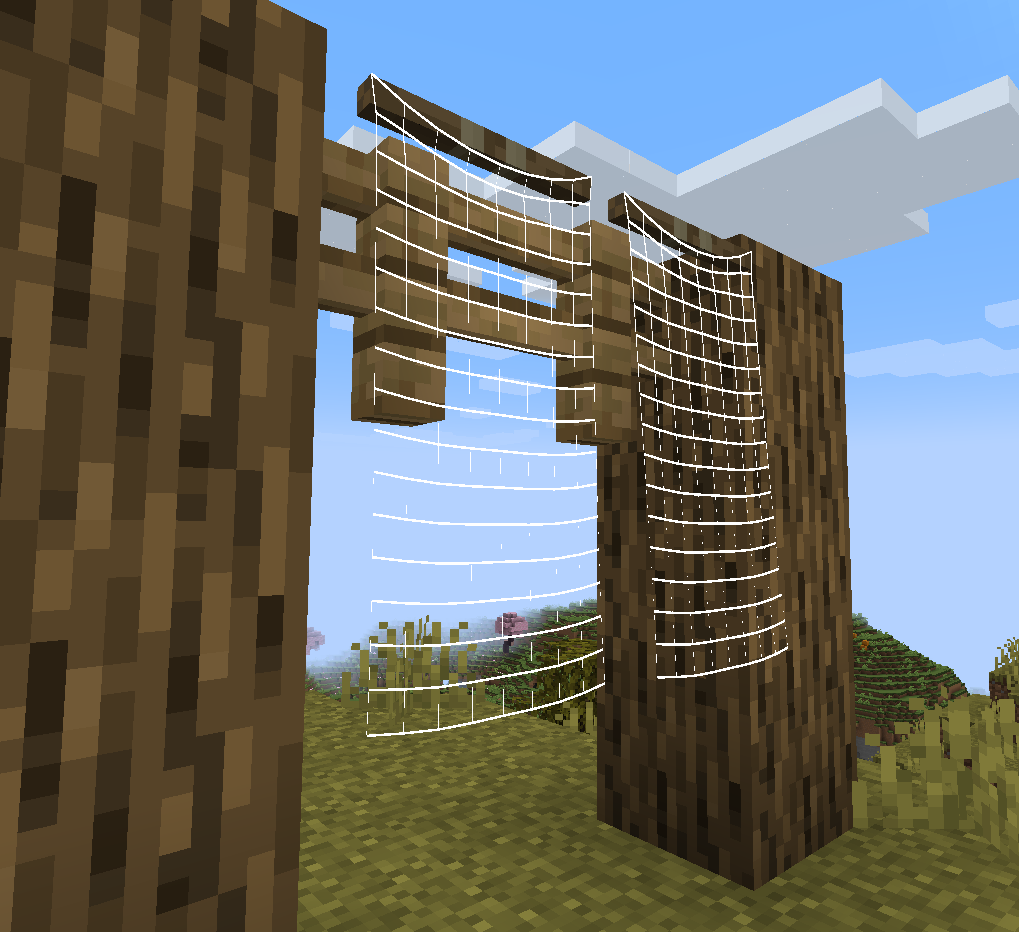
\includegraphics[height=2.75in]{images/bannermidgridwf.png}
        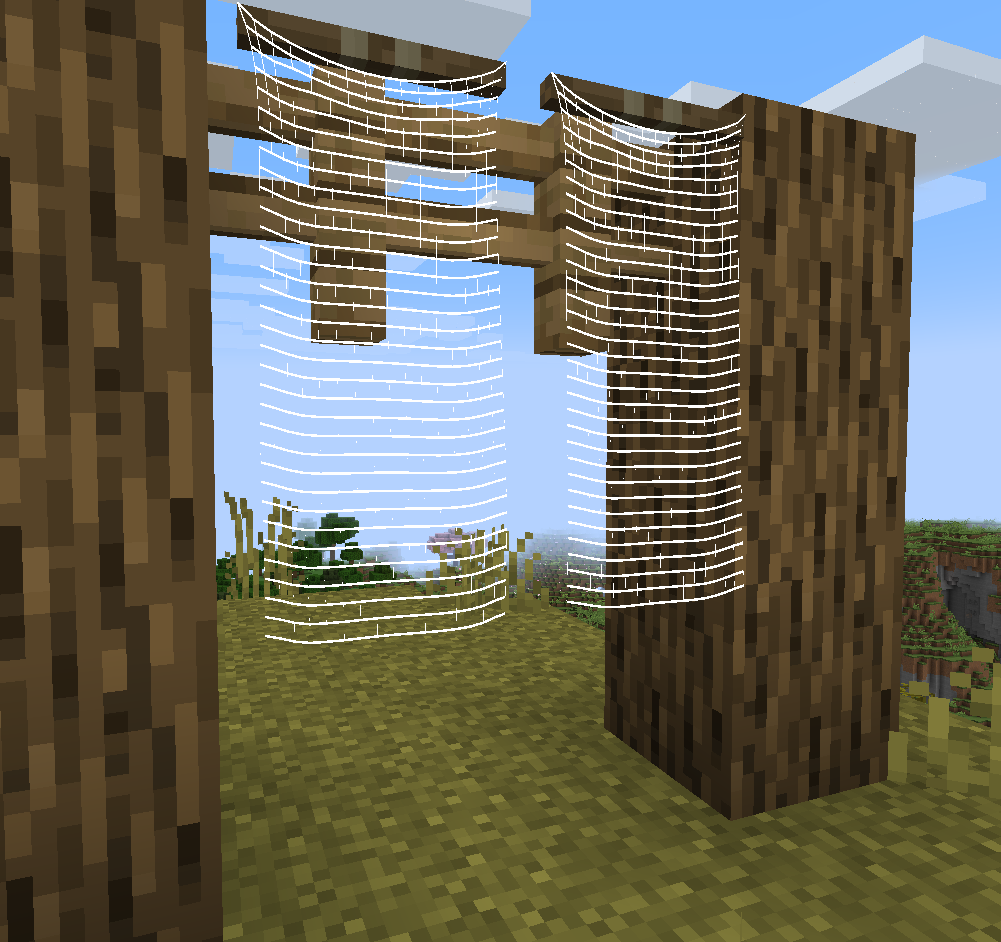
\includegraphics[height=2.75in]{images/bannerlargegridwf.png}
    \end{center}
    \caption{Banner wireframes with larger grids.}
\end{figure}

\begin{figure}[hp]
    \begin{center}
        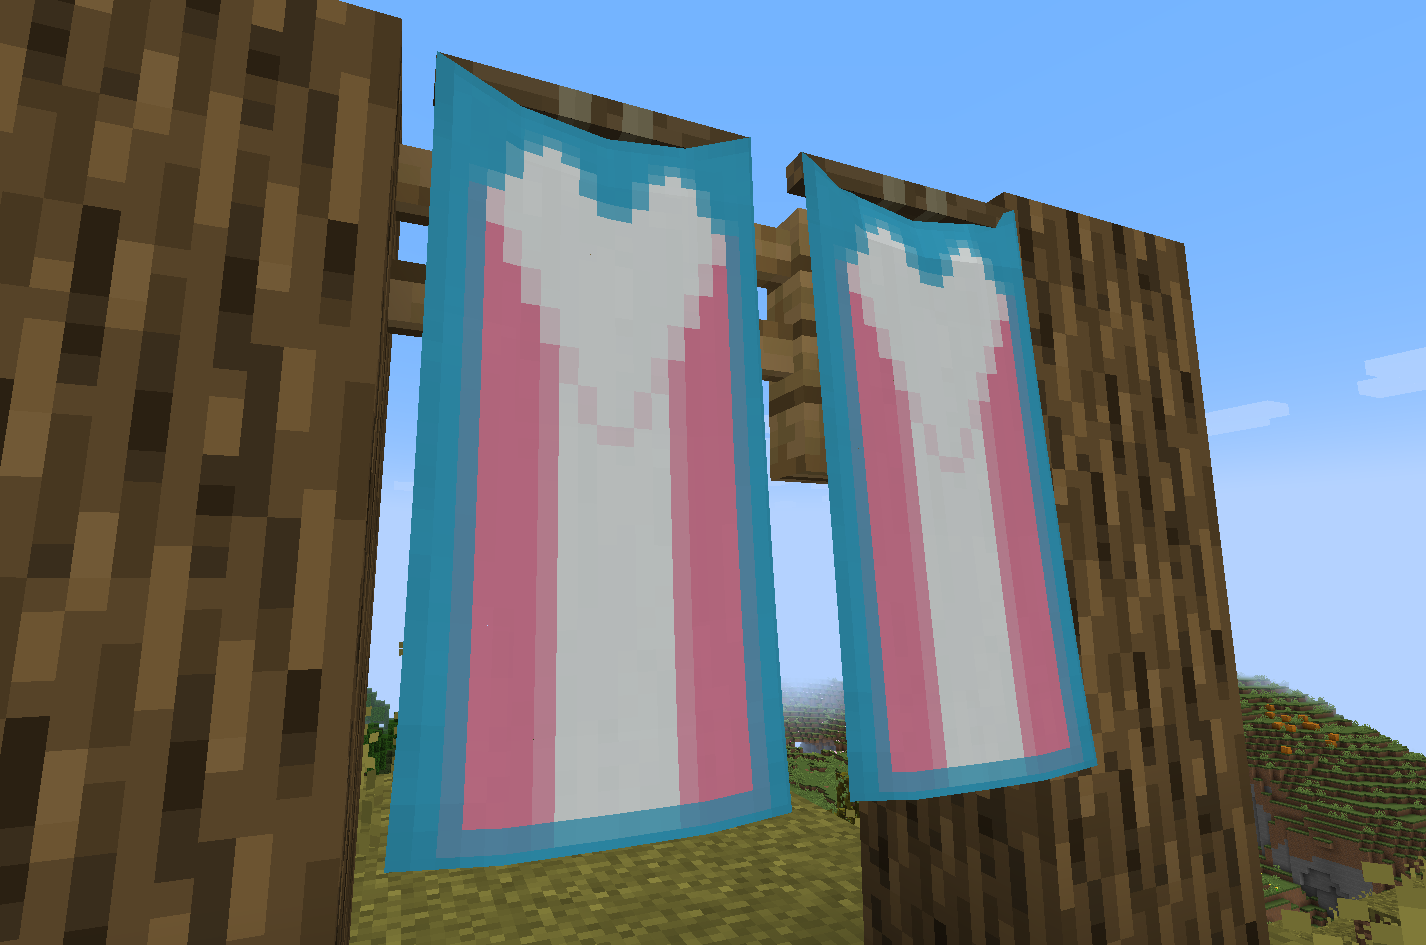
\includegraphics[width=3in]{images/transbanners.png}
        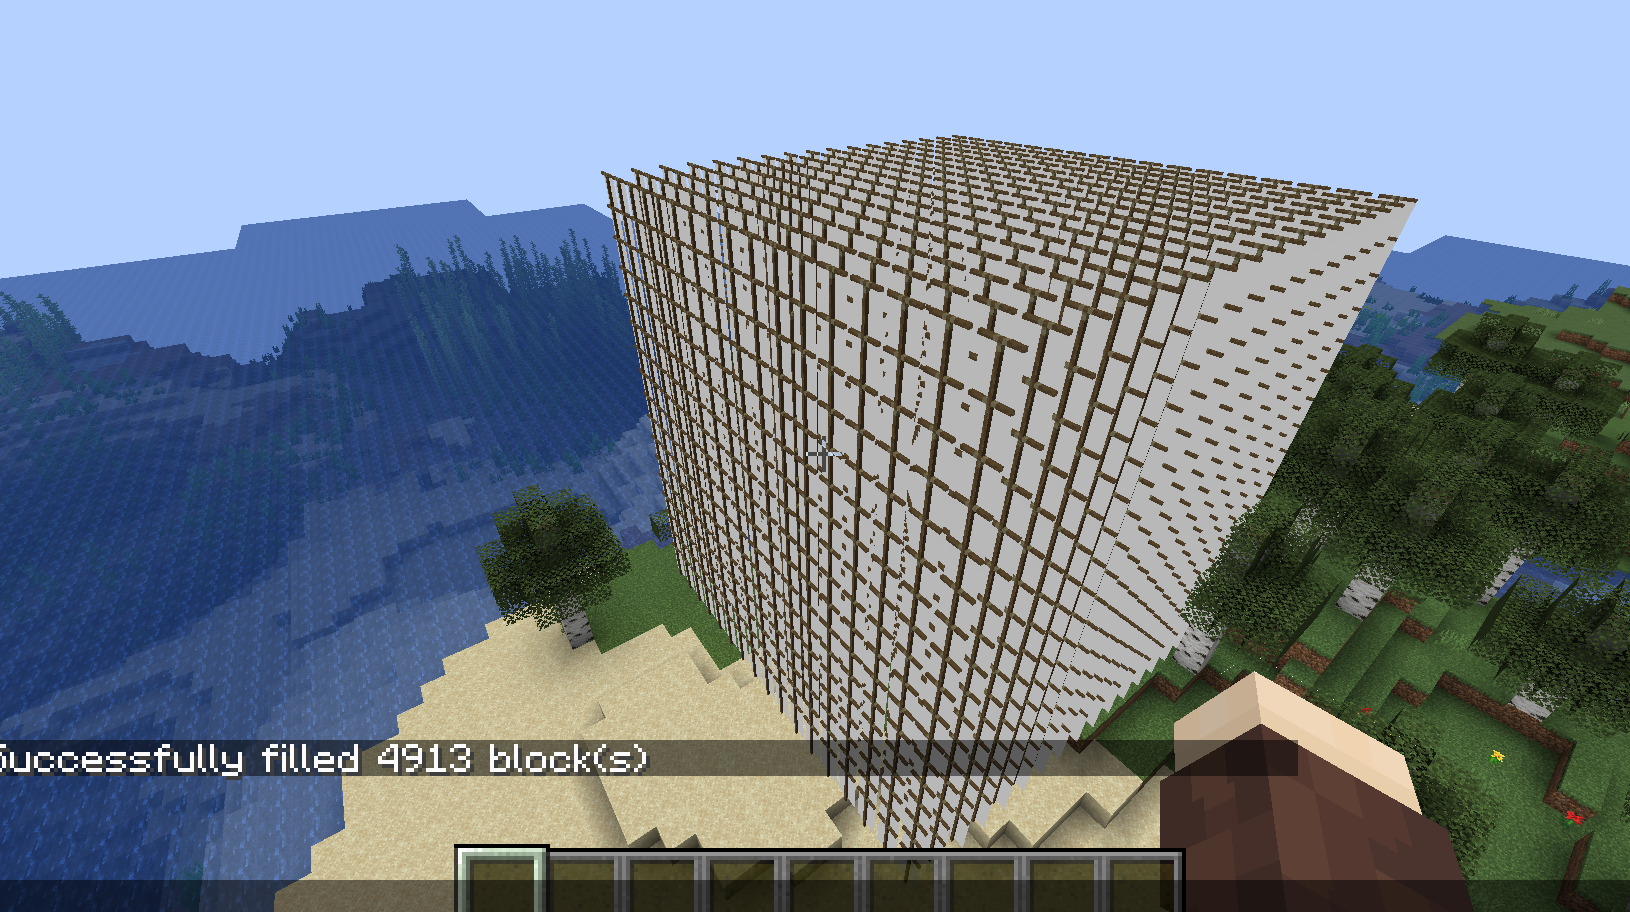
\includegraphics[width=3in]{images/4913stresstest.png}
    \end{center}
    \caption{Left: Textured banners. Right: Banner stress test with 4913 banners.}
\end{figure}

\section{Conclusion}

While the current form of this project falls quite short of its initial goals, it's still a great first step! We now have a solid core cloth algorithm working in game with relatively good performance. Next steps will be to build a proper API around it, extend it to more easily support a variety of shapes, properly integrate it with the game world, and continue exploring ways to better match the game's style.\\
\\
And of course, the final step will be to make skirts with it, but it looks like that's a ways away still perhaps.


\bibliography{reportrefs}

\end{document}